\documentclass[a4j,dvipdfmx]{jarticle}
%----------------------------------------------------------------------
\usepackage{graphicx}
%\usepackage{amsmath}
%\usepackage{amssymb}
%\usepackage{bm}
%\usepackage{fancybox}
\usepackage{fancyhdr}
\usepackage{lastpage}
%\usepackage{color}
\usepackage{multicol}
\usepackage{listings,jlisting}
\usepackage{ascmac}
%----------------------------------------------------------------------
%\setlength{\topmargin}{-0.5in}
%\addtolength{\headheight}{1cm}
%%\setlength{\headsep}{0mm}
%\setlength{\oddsidemargin}{-0.5in}
%%\setlength{\evensidemargin}{-0.5in}
%\addtolength{\textwidth}{1.5in}
%\addtolength{\textheight}{1in}
%----------------------------------------------------------------------
%\setlength{\columnsep}{2zw}
%\setlength{\columnseprule}{0.4pt}
%----------------------------------------------------------------------
\pagestyle{fancy}
\lhead{2016/07/19}
\rhead{配布資料(\thepage / \pageref{LastPage})}
\cfoot{}
\chead{\textgt{システムプログラミング2 第13回}}
%----------------------------------------------------------------------
\begin{document}
\def\lstlistingname{リスト}
\lstset{language=C,
  numbers=none,
  basicstyle={\small\ttfamily},
  columns=[l]{fullflexible},
  keepspaces=true,
  frame=shadowbox,
  commentstyle=\slshape
}
%----------------------------------------------------------------------

%\begin{figure}[hbtp]
%\begin{center}
%\includegraphics[height=2.5cm]{state.pdf}
%\caption{単語の長さをカウントするアルゴリズム}
%\end{center}
%\end{figure}

今回は、プログラムで他のプログラムを起動する方法を学ぶ。
プログラムを起動する方式には大きく分けて、
{\bf spawn方式}(スポーン:卵を産む)と、
{\bf fork-exec方式}(分岐-実行?)がある。

\begin{enumerate}

\item spawn 方式

Windows等で使用される方式である。
新しい「(1) プロセスを作り」、
「(2) プログラムを実行する」の二つの仕事を
一つのspawnシステムコールで行うので分かりやすい。

fork-exec方式を実現するためには、
メモリ再配置のためのハードウェア機構をCPUが持っている必要がある。
そのため組込用の小さなコンピュータ等ではspawn方式しか選択肢がない場合がある。

最近のUNIX系のOSではspawn方式も使用できるようになっている。
次にMacの\verb/posix_spawn/システムコールを紹介する。

\begin{lstlisting}[numbers=none]
書式: #include <spawn.h>
       int posix_spawn(int * pid, char *path,
         posix_spawn_file_actions_t *file_actions,  posix_spawnattr_t *attrp,
         char * argv[restrict], char * envp[restrict]);

解説: 新しいプロセスを作り path で指定したプログラムを実行する。
       pid は新しいプロセスのプロセス番号を格納する変数を指すポインタ。
       file_action, attrp はプロセスの初期化を指示するデータ構造へのポインタ。
       argv, envp は実行されるプログラムの main 関数の argv, envp に渡すデータ。
\end{lstlisting}


\item fork-exec 方式

UNIX系のOS用いられてきた方式のこと。
まず「(a) 新しいプロセスを作り(forkシステムコール)」、
次にユーザが記述したプログラムで初期処理を行い、
最後に「(b) 新しいプログラムをロード・実行(execシステムコール)」する。
初期化処理をユーザが自由にプログラムで記述できるので柔軟性が高い。

\begin{enumerate}
\item プログラムをロード・実行(execシステムコール)

プロセスが新しいプログラムの実行を開始するシステムコールである。
プロセスが新しいプログラムを実行するプロセスに変身する(変身の術)。
以下に、UNIXのexecシステムコール(\verb/execve/システムコール)の解説を示す。

\begin{lstlisting}[numbers=none]
書式: #include <unistd.h>
       int execve(char *path, char *argv[], char *envp[]);

解説: 自プロセスで path で指定したプログラムを実行する。
       argv, envp は実行されるプログラムの main 関数の argv, envp に渡すデータ。
       正常時には execve を実行したプログラムは新しいプログラムで上書きされる。
       execveシステムコールが戻る(次の行が実行される)のはエラー発生時だけである。
\end{lstlisting}


\begin{figure}[hbtp]
\begin{center}
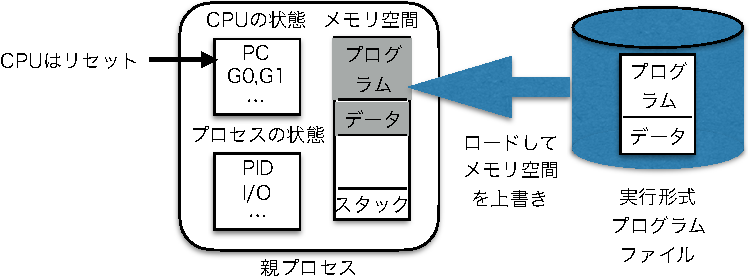
\includegraphics[scale=0.8]{exec-crop.pdf}
\caption{execの仕組み}
\label{fig_exec}
\end{center}
\end{figure}

図\ref{fig_exec}に\verb/exec/システムコールを実行するプロセスの様子を示す。
プロセスが\verb/exec/システムコールを実行すると、
そのプロセスのメモリ空間に新しいプログラムが実行形式ファイルからロードされる。
\verb/exec/システムコールを実行したプログラムは、
新しいプログラムで上書きされる。
プロセスの仮想CPUはリセットされ、
新しいプログラムの実行が開始される。

リスト\ref{exectest1}に\verb;execve;システムコールを使用して、
\verb;/bin/date;プログラムを実行するプログラムの例を示す。

\lstinputlisting[label=exectest1, caption=execveの使用例(その1)]{exectest1.c}

リスト\ref{exectest3}は、
環境変数の一部を書き換えた上で、
\verb;/bin/date;プログラムを実行するプログラムの例である。

\lstinputlisting[label=exectest3, caption=execveの使用例(その2)]{exectest3.c}

リスト\ref{exectest2}は、
全く新しい環境変数の一覧を渡して
\verb;/bin/date;プログラムを実行するプログラムの例である。

\lstinputlisting[label=exectest2, caption=execveの使用例(その3)]{exectest2.c}

リスト\ref{exectest4}は、
複数のコマンド行引数がある場合の例である。
\verb;/bin/echo;プログラムを``aaa''、``bbb''を引数にして実行する。
\verb;args;配列にプログラムの名前(argv[0]:``echo'')を
忘れないように注意すること。

\lstinputlisting[label=exectest4, caption=execveの使用例(その4)]{exectest4.c}

execする際、プロセス状態の一部は引き継がれる。
例えば、オープン中のファイルや、
「無視」に設定されたシグナルハンドリング等は、
新しいプログラムがロードされてもそのまま引き継がれる。
この仕組みを使用して、
プログラム実行開始前に標準入力(0)、標準出力(1)、
標準エラー出力(3)がオープンされる。

シェルはfork-execを使用してプログラム(外部コマンド)を起動している。
シェルのリダイレクト(プログラムの入出力を切替える仕組み)は、
リダイレクト先のファイルを標準入力・出力としてオープンした状態で
外部プログラムをexecすることで実現できる。
リスト\ref{exectest5}は、
標準出力を``aaa.txt''にリダイレクトした状態で
\verb;/bin/echo;を実行するプログラムである。

\lstinputlisting[label=exectest5, caption=execveの使用例(その5)]{exectest5.c}

\item 新しいプロセスを作る(forkシステムコール)

\verb/exec/システムコールはプロセスを新しいプログラムに変身させる。
変身して新しいプログラムを実行したプロセスは終了してしまう。
新しいプロセスを作って、新しいプログラムを実行させる仕組みが必要である。
\verb/fork/システムコールは新しいプロセスを作成し自身をコピーする。
つまり、{\bf 分身}を作るシステムコールである(分身の術)。

\begin{lstlisting}[numbers=none]
書式: #include <unistd.h>
       int fork(void);

解説: プロセスのコピーを作る。親プロセスには子プロセスのPIDが返される。
       エラー時は、親プロセスに-1が返され子プロセスは作られない。
\end{lstlisting}

\verb/fork/システムコールを実行した「プロセスがコピーされ」る。
元のプロセスを{\bf 親プロセス}、
コピーして作ったプロセスを{\bf 子プロセス}と呼ぶ。
図\ref{fig_fork}にforkの様子を、
リスト\ref{forktest}に\verb/fork/システムコールを実行するプログラムの例を、
以下にforkの処理手順を示す。

\begin{enumerate}
\item 親プロセスがプログラム実行中に\verb/fork/システムコールを実行する。
\item 新しいプロセス(子プロセス)が作られ、親プロセスの内容がコピーされる。
\item 子プロセスには、
メモリ空間(プログラム、変数(データ)、スタック)、
プロセスの状態(どのファイルをオープン中か、シグナルハンドラの登録等)、
CPUの状態(CPUレジスタの値、SPの値、PCの値、フラグの値)等、
全ての情報がコピーされる。
ただし、プロセス番号(PID:Process ID)値は親子プロセスで異なる。
\item 親プロセスは\verb/fork/システムコールを終了しプログラムの実行を再開する。
この時、\verb/fork/システムコールは子プロセスのPIDを返す。
\item 子プロセスは\verb/fork/システムコールを呼出した瞬間のコピーなので、
\verb/fork/システムコールが終了するところからプログラム実行を開始する。
この時、\verb/fork/システムコールは\verb/0/を返す。
\end{enumerate}

最終的に親プロセスと子プロセスが同時に並行して実行される状態になる。

\begin{figure}[hbtp]
\begin{center}
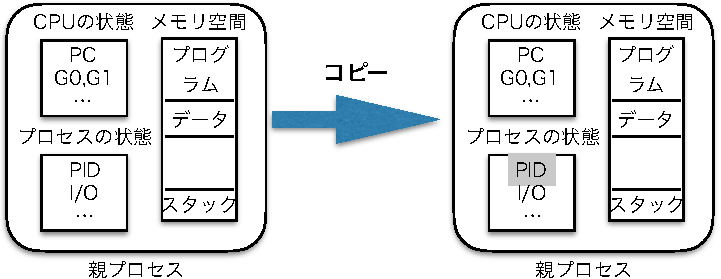
\includegraphics[scale=0.8]{fork-crop.pdf}
\caption{forkの仕組み}
\label{fig_fork}
\end{center}
\end{figure}

\lstinputlisting[label=forktest, caption=forkの使用例]{forktest.c}

\end{enumerate}

% プロセスが同時に並行して処理ができることを利用して、
% 複数のプログラムを組み合わせて一つの処理をさせるような応用が可能である。
% 例えばパイプがそうである。
% 以下の例では\verb/sort/プロセスの出力と
% \verb/grep/プロセスの入力が接続された状態で、
% 二つのプロセスが同時に実行される。

% \begin{lstlisting}[numbers=none]
% $ cat a.txt
% kobayasi
% momota
% yamada
% yosinaga
% okumoto
% sigemura
% $ sort  a.txt | grep i        # a.txt をアルファベット順にソートし i を含む行だけ出力
% kobayasi
% sigemura
% yosinaga
% \end{lstlisting}

\item プロセスの終了と待ち合わせ

親プロセスは子プロセスを幾つか作成しそれらに同時に並行して処理を行わせる。
子プロセスは処理を終えると終了する。
子プロセスが処理を終えると
親プロセスは各子プロセスが正常に終了したかチェックする。
全ての子プロセスが正常に終了していれば処理全体が完了である。
このような処理ができるように、
子プロセスが処理結果と共に自身を終了する\verb/exit/システムコールと、
親プロセスが子プロセスの終了を待つ\verb/wait/システムコールが準備されている。
(正確には\verb/exit/は\verb/_exit/システムコールを呼び出すライブラリ関数)

子プロセスは\verb/exit/システムコールを実行してもすぐに消滅するわけではない。
子プロセスは、
親プロセスが\verb/wait/システムコールを実行して終了ステータスを取り出して
くれるまで待ち状態になる。
この状態をzombi状態と呼ぶ。

なおCプログラムの\verb/main/関数は、スタートアップルーチンから
\verb/exit(main(argc, argv, envp));/のように呼び出されている。
\verb/main/関数を\verb/return n;/で終了すると、
\verb/exit(n);/が実行されることになる。
つまり、
\verb/main/関数中では\verb/return n;/と\verb/exit(n);/が同じ意味になる。

\begin{lstlisting}[numbers=none]
書式: #include <stdlib.h>
       void exit(int status);

解説: 自プロセスを終了する。親プロセスは wait システムコールで status の値を受け取る。
       終了ステータス(status)は下位 8bit が有効である。(0 <= status <= 255)
       exit を呼び出すとプロセスが終了するので exit は戻らない。
\end{lstlisting}

\begin{lstlisting}[numbers=none]
書式: #include <sys/wait.h>
       void wait(int *status);

解説: 子プロセスの終了を待つ。status に子プロセスが終了した理由等が格納される。
       status の下位 8bit には、子プロセスが exit に渡した終了ステータスが格納される。
       その他のビットで終了の理由(exit、シグナル等)が分かるようになっている。
\end{lstlisting}

\item fork-exec方式のプログラム例

リスト\ref{forkexec1}に
新しいプロセスで新しいプログラムを実行するプログラムの基本的な例を示す。
このプログラムは、
\verb/fork/、\verb/exec/、\verb/exit/、\verb/wait/を組み合わせて
使用する一般的な例である。
図\ref{fig_forkexec}は、
リスト\ref{forkexec1}のプログラムの動きを解説したものである。

\begin{figure}[hbtp]
\begin{center}
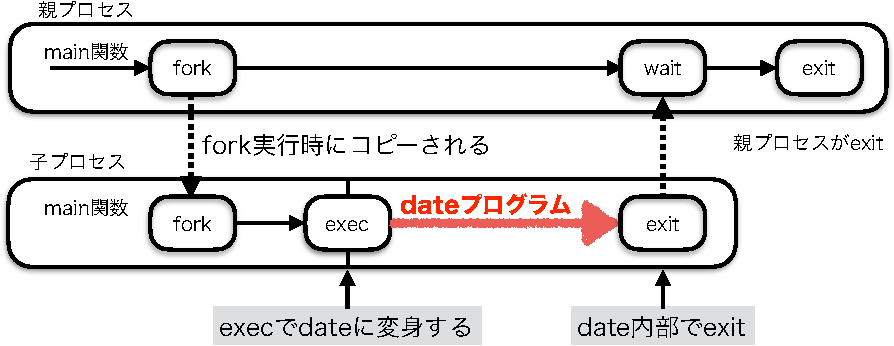
\includegraphics[scale=0.8]{fork-exec-crop.pdf}
\caption{fork-execの仕組み}
\label{fig_forkexec}
\end{center}
\end{figure}

\lstinputlisting[label=forkexec1, caption=fork-execの例]{forkexec1.c}

リスト\ref{forkexec2}に少し実用的な例を示す。
このプログラムは、実行例に示すようにコマンド行引数に
指示された環境変数の変更を行った上でdateプログラムを次々に実行する。
環境変数の変更は子プロセス側で行うようになっているので、
親プロセスの環境変数は変化しない。


\lstinputlisting[label=forkexec2,
caption=子プロセスで環境変数を次々変更しながらdateを次々実行]{forkexec2.c}

リスト\ref{forkexec3}は、
環境変数の変更を親プロセスが\verb/fork/前に行うように変更したものである。
リスト\ref{forkexec2}の実行結果との違いに注目して欲しい。

\lstinputlisting[label=forkexec3,
caption=親プロセスで環境変数を次々変更しながらdateを次々実行]{forkexec3.c}

\item 問題

コマンド行引数で「環境変数とファイル名」の組を複数指定し、
環境変数を変更した上で出力をファイルにリダイレクトしdateを実行する
プログラムを作りなさい。
例えば次のように実行すると、現在時刻をキューバ時間で表したものが\verb/c.txt/に
ローマ時間で表したものが\verb/r.txt/に格納される。

\verb;$ a.out TZ=Cuba c.txt TZ=Europe/Rome r.txt;

\end{enumerate}
\end{document}
